\section{Evaluation}
\label{sec:eval}
In this section, we first give some statistics of our 
corpus, and evaluate the quality of our extracted 
cause-effect causal training pairs.
We then introduce two evaluation datasets and 
a bunch of evaluation metrics we adopted in our experiments. 
Next, we compared our results on the commonsense causality generation task against a number of baselines. 

\subsection{Datasets}
\label{sec:datasets}
We first describe the text corpus we used for 
cause-effect pairs extraction, and then introduce
two evaluation datasets for the following experiments.

\subsubsection{Novel Corpus}
\label{sec:novel_corpus}
Novels created by writers are high quality text sources.
Recent works~\cite{gordon2011commonsense, trinh2018simple} show that the data of stories texts from novels and books benefit the commonsense reasoning tasks more than other sources.
Thus, we use a large number of novels 
which are a good source of commonsense causal information as our text corpus for the cause-effect pairs extraction. 

We first crawl raw novel corpus from Library Genesis\footnote{\url{libgen.is}}, a search engine for articles and books which allows free access. 
%\SN{This website seems have repeated got into copyright disputes, need check if it's good to mention it here.} 
To maintain the quality of our corpus, we collect a group of prize-winning lists and top-x lists for novels, for example Nobel Prize in Literature and Time Magazine All Time 100 Novels, and limit our crawler to them. The resulting 19000 novels are splitted into around 100 million sentences, which served as our data source after filtering and text cleaning. 

We perform the cause-effect pairs extraction process on
the crawled corpus (described 
in~\secref{sec:causal_pairs}). 
Each pair can be transformed into two examples
following the input transformation as described in ~\figref{fig:example}. 
Finally, we obtain 539,930 cause-effect example pairs from novels. We split them into training split (431,944 examples, 80\%), validation split (53,993 examples, 10\%),
and test split (53,993 examples, 10\%).

%
%For causal pair extraction, we first collect sentences containing ``because'' or ``so'' by regular expression matching. Those sentences are fed into Stanford CoreNLP~\cite{stanfordcorenlp} tools for tokenization, POS tagging, constituent parsing, dependency parsing and coreference annotation. Following steps are taken to filter out syntactically unwanted or semantically non-causal pairs and to locate the right span of target content:
%\begin{figure}[t!]
%	\centering
%	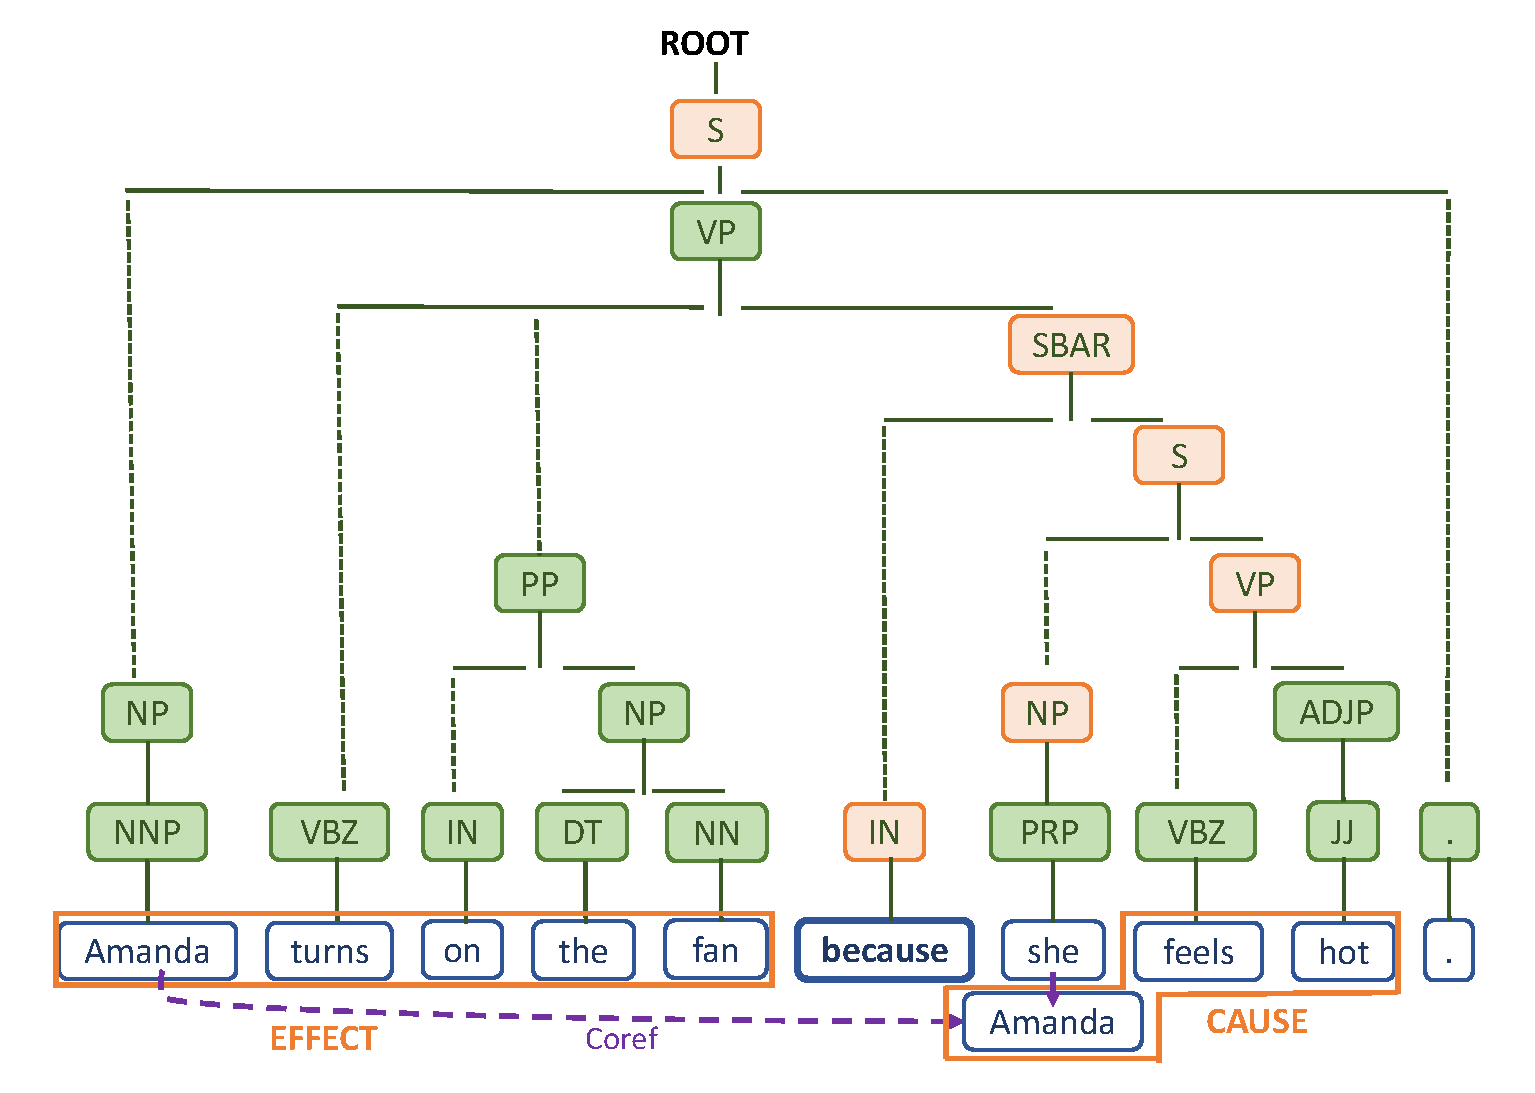
\includegraphics[width=\columnwidth]{parse.pdf}
%	\caption{Cause and effect sentence extracted from a sample sentence along with its constituent parse tree. Nodes coloured in light orange are those critical for syntactical checking in our extraction process.}
%	\label{fig:parse}
%\end{figure}
%\begin{itemize}
%	\item Negation Detection. If the causal conjunction node in dependency tree
%	 has a negation word sibling such as ``not'' and ``n't'', causal relationship 
%	 doesn't exist in this sentence.
%	\item Clause Detection. Since the input and target of our task are both sentences, 
%	cause or effect represented by noun phrases are unwanted. For example, "This is 
%	because of you" has noun as both cause and effect, thus doesn't satisfy our 
%	requirement. We design complicated pattern matching rules on dependency parse 
%	tree and constituent parse trees for this syntactic checking. A simple sample 
%	sentence with its constituent parse tree is shown in \ref{fig:parse}. Basically 
%	we make sure the "because" in the sentence is a subordinate conjunction word 
%	leading a subordinate clause(tagged as `SBAR'), which contains a declarative 
%	sentence(`S') with subject(`NP') and predicate(`VP'). \SN{not complete here. 
%		Jessie may want to say may about this.}
%	\item Span Selection. Sentences passing the previous steps must already have 
%	main clause root node and subordinate clause root node identified in constituent 
%	parse tree. In this step we confirm the spans of cause/effect sentence based on 
%	the root nodes' spans to remove punctuations and unwanted  sentence constituents.
%	\item (Partial) Coreference Resolution. The order of cause/effect span is determined by the 
%	causal conjunction. Take ``because'' as an example, the order is always ``EFFECT 
%	because CAUSE'', resulting in representative mention in effect sentence but 
%	pronouns in cause. Therefore, we substitute pronouns in subordinate clause with 
%	the representative mention in main clause for each causal pair to enable bidirectional 
%	inference. We don't do coreference resolution on the whole sentence to avoid unnecessary repetition. 
%\end{itemize}
%After performing those steps to all sentences in novel corpus, we get \SN{477644} unique 
%cause-effect pairs. \SN{maybe more statisticas here?}

\subsubsection{Evaluation Datasets}
For the causality generation task, two evaluation datasets are used in the following evaluation experiments.

\textbf{Novel.}
We use the test split in~\secref{sec:novel_corpus} as the first evaluation dataset.
The novel test split contains 53,993 examples, and are
from the same data source with the training data.
The specific examples are formated as shown in~\figref{fig:example}. 

\textbf{ COPA.}
To better understand the performance of our model against related research, we also use 
the Choice of Plausible Alternatives (COPA) 
as test dataset, which is a widely-attempted causal reasoning benchmark. It consists
of one thousand multiple-choice questions.
Each question is composed of a premise and two alternatives,
where the task is to select the more plausible alternative as a cause (or effect) of the premise. 
We do the input transformation on each question, 
which puts the special token $\left< f\right>$ or $\left< b\right>$ in front of the premise or alternative to form a cause-effect sequence pair.
We use the test split in~\cite{gordon2011commonsense}
which contains 500 questions.
After the input transformation,
the built COPA evaluation dataset consists of 1000 cause-effect pairs. 


\subsection{Baselines}
There are five baselines in the evaluation experiments
which can be divided into two categories:
the selection-based methods and the generation-based methods. 
In this section, we describe those baselines in details.

\subsubsection{Selection-based}
To perform the causality generation task, the selection-based models first automatically generate a set of target candidates $C^t$ for the given source $s$, then
select the best answer from those candidates to reason about causalities. 
Basically, given the source $s$, we automatically
match $s$ with the sources extracted from the novel 
corpus and select 10 most similar sources constituted $C^s$. 
Then, the set of target candidates $C^t$ is composed by the corresponding target of each source in $C^s$.
Then we compute the causal strength between 
$s$ and each $t$ in $C^t$ to select the best answer 
and generate it as the target.
We design three selection-based baselines as follows,
among which the main difference is 
the matching approach when generating the candidates set $C^s$ for $s$.

\textbf{Unigram-1.}
We use the unigram overlaps between the given source $s$ and all the sources in the extracted corpus to select 10 most similar sources as $C^s$.

\textbf{Unigram-2.}
Unigram-2 baseline is similar to Unigram-1 except that
we remove the stopwords from the sources.

\textbf{Bigram.}
Bigram baseline is similar to Unigram-1 except that
we use the bigram instead of the unigram for the
candidates set generation.

\subsubsection{Generation-based}
Generation-based methods for causality generation
are all based on the CNN encoder-decoder sequence to sequence model. These baselines can directly generate
the causalities without $C^t$ selection step in
selection-based baselines.

\textbf{CNN Seq2seq with soft attention.}
We use the conventional CNN seq2seq model as the
baseline, which is effective,  validated~\cite{DBLP:conf/emnlp/EdunovOAG18,DBLP:conf/coling/SongTHLQL18,DBLP:journals/corr/abs-1809-10853, DBLP:conf/acl/LewisDF18} and fully parallelized.
The CNN with soft attention baseline is described in~\secref{sec:cnn}.

\textbf{CNN Seq2seq with causal attention.}
We substitute the proposed causal attention for the soft attention in CNN seq2seq model.
We detailedly explain the proposed causal attention in ~\secref{sec:causal_attention} 

%Others are introduced in \secref{sec:approach}:
%causality strength between them and premises, and select cause (or effect)
%with best causality strength score.
%There are four baselines in our experiments.
%One is to select causes (or effects) based on premise 
%from Cause-Effects Pairs Corpus. 
%In details, given a premise and its attribute (cause or effect), 
%we rank premises with the same attribute as given premise
%in Cause-Effects Pairs Corpus by cosine similarity 
%and select top $10$. We can get corresponding causes (or effects)
%of these $10$ premises. We rank these causes (or effects) by
%causality strength between them and premises, and select cause (or effect)
%with best causality strength score.
%Others are introduced in \secref{sec:approach}:
%CNN seq2seq model and causal attention.



\subsection{Evaluation Metrics}
\label{sec:metrics}
In this section, we introduce the evaluation metrics used in 
our experiments.

\textbf{BLEU} scores~\cite{PapineniRWZ02}, 
includes BLEU-1 (B-1), BLEU-2 (B-2) and BLEU-3 (B-3)
which combines modified n-gram precisions and sentence brevity penalty:

\begin{equation}
\small BLEU = \min(1,\exp(1-\frac{r}{c})) \cdot \sum_{n=1}^{N}(w_{n}p_{n})
\end{equation}

where $r$ is the sum of the best match lengths 
for each generated and corresponding reference text in the corpus.
and $c$ is the total length of the predicted corpus. 
$w_n=\frac{1}{N}$ is uniform weights. $N$ is based on the type of BLEU, 
for example, $N$ is $2$ for BLEU-2
$p_n$ is modified n-gram precision. To compute this, 
one first counts the maximum number of times a word occurs reference text. 
Next, one clips the total count of each predicted word by its maximum
reference count, adds these clipped counts up, and
divides by the total number of predicted words. 

%\textbf{Causality Score for Text} (CST) from predicted text $T_1$
%and premise text $T_2$ is computed as \cite{LuoSZHW16}:
%
%\begin{equation}
%\small cst(T_{1},T_{2}) = -\log(\frac{\sum_{i \in T_{1}}\sum_{j \in T_{2}}cs(i,j)}{\left| T_{1} \right| + \left| T_{2} \right|})
%\end{equation}
%\begin{equation}
%\small CST(T_{1},T_{2}) = \frac{1}{cst{T_1,T_2}}
%\end{equation}
%where $cs(i,j)$ is causality strength 
%between $i$-th token in $T_1$ and $j$-th token in $T_2$. 
%The higher the score, the stronger the causality.

\textbf{Accuracy} (Acc) is evaluation metric for COPA.
We generate cause (or effect) according to the premise in COPA
and select the more ``similar'' alternative based on the similarity
score. We use \textbf{BLEU} as similarity evaluation methods.

\begin{equation}
Acc = \frac{n_{ct}}{N_{all}}
\end{equation}
where $n_{ct}$ and $N_{all}$ denotes
the number of the questions with correct selection
and all questions in COPA respectively.

We use BLEU-1 since it is suitable for generation
of short sequence. It denotes the degree of matching 
predicted texts and premise texts. 
%As relation between cause and effect is many-to-many, 
%we use CS score, which denotes the causality, to supplement
%BLEU-1 score. The reason for using BLEU and CS as similarity
%score is that they respectively indicate the consistency and causality 
%between two text.

\textbf{Human Evaluation} (Human) is used to supplement
BLEU-1 score, as relation between cause and effect is many-to-many.
We randomly sample 100 generated cause-effect pairs of COPA
and sample 300 generated cause-effect pairs of novel
by each model.
We manually inspect whether there is a correct causality between source sequence
and generated sequence.
Then, we calculate the percentage of the generated 
cause-effect pairs with correct causality in each model.
This estimate the 
ability of models to generate correct causes (or effects) based on permise .

\subsection{Experiments}
\label{sec:exp}
In this section, we compare the results of our model
against five baselines on the causality generation task.
We evaluate them on two evaluation datasets (described in~\secref{sec:datasets}) using four evaluation metrics
(described in~\secref{sec:metrics}).

We train generation-based baselines as well as our model
on the training split of novel corpus.
It is natural to evaluate on the test split of novel corpus.
To show the effectiveness and well generality of our model, we also perform the evaluation 
on COPA, a public commonsense causal reasoning dataset.
We straightforwardly fine-tune models with a minimal COPA dev split which contains 500 questions.
As shown in ~\tabref{tab:novel} and ~\tabref{tab:copa}, 
the proposed model CNN+CSFusion outperforms 
all the baselines on every evaluation metrics
except the bleu-1 score on COPA test.
%Since Bleu-1 scores mainly consider the unigrams in the generated target.

\begin{table}[th]
	\centering
	\begin{tabular}{|l|c|c|c|c|c|}
		\hline
		Model &   B-1  & B-2 & B-3 & Human \\
		\hline
		CS  & 15.96 & 0.61 & 0.04 & 0.18 \\
		CNN & 23.64 & 4.06 & 0.92 & 0.21 \\
		\hline
		CNN+CSFusion & \bf 24.53 & \bf 4.07 & \bf 0.94 & \bf 0.35 \\
		\hline
	\end{tabular}
	\caption{BLEU score and Causility strength score on Cause-Effect Pairs Corpus}
	\label{tab:novel}
\end{table}

\begin{table}[th]
	\centering
    \small
	\begin{tabular}{|l|c|c|c|c|c|c|}
		\hline
		Model &   B-1 & B-2 & B-3 & Human\\	\hline
        unigram-1 & 11.15 & 0.14 & 0.0 & 0.26 \\\hline
        unigram-2 & 12.35 & -  & - & 0.17 \\\hline
        bigram & 13.42 & 0.41 & 0.0 & 0.26 \\\hline
		CS & 18.90 & 0.12 & 0.0 & 0.21 \\\hline
		CNN & \bf 42.14 & 17.19 & 2.10 & 0.25 \\\hline
		CNN+CSFusion & 40.60 & \bf 17.51 & \bf 2.31 & \bf 0.52 \\\hline
	\end{tabular}
	\caption{BLEU score, Causality strength score and Accuracy on COPA}
	\label{tab:copa}
\end{table}

\cut{%%%
\begin{table}[th]
	\centering
    \small
	\begin{tabular}{|l|c|c|c|c|c|}
		\hline
		Model &   B-1  & B-2 & B-3 & CST & Human \\
		\hline
		CS  & 15.96 & 0.61 & 0.04 & 1.59 & 0.18 \\
		CNN & 23.64 & 4.06 & 0.92 & \bf 1.87 & 0.21 \\
		\hline
		CNN+CSFusion & \bf 24.53 & \bf 4.07 & \bf 0.94 & 1.77 & \bf 0.35 \\
		\hline
	\end{tabular}
	\caption{BLEU score and Causility strength score on Cause-Effect Pairs Corpus}
	\label{tab:novel}
\end{table}

\begin{table}[th]
	\centering
    \small
	\begin{tabular}{|l|c|c|c|c|c|c|}
		\hline
		Model &   B-1 & B-2 & B-3 & CST & Human\\	\hline
        unigram-1 & 11.15 & 0.14 & 0.0 & 2.42 & 0.26 \\\hline
        unigram-2 & 12.35 & -  & - & 2.80 & 0.17 \\\hline
        bigram & 13.42 & 0.41 & 0.0 & 2.50 & 0.26 \\\hline
		CS & 18.90 & 0.12 & 0.0 & 2.27 & 0.21 \\\hline
		CNN & \bf 42.14 & 17.19 & 2.10 & \bf 1.93 & 0.25 \\\hline
		CNN+CSFusion & 40.60 & \bf 17.51 & \bf 2.31 & 1.83 & \bf 0.52 \\\hline
	\end{tabular}
	\caption{BLEU score, Causality strength score and Accuracy on COPA}
	\label{tab:copa}
\end{table}

\begin{table*}[th]
    \centering
    \small
    \begin{tabular}{|r|l|}%{|p{7cm}|rl|}
    \hline
    \multicolumn{2}{|c|}{Cause}\\ 
    \hline
    \multicolumn{2}{|c|}{you were the only one that wanted me to win}\\ 
    \hline
    \multicolumn{2}{|c|}{Effect} \\
    \hline
    \multicolumn{2}{|c|}{i came to you}\\ 
    \hline
    CS & i was n't sure \\
    \hline
    CNN & i was not going to fight you \\
    \hline
    CNN+CSFusion & i was a little worried \\
    \hline
    \end{tabular}
    \caption{Given cause to generate effect.}
    \label{tab:cause_exp}
\end{table*}

\begin{table*}[th]
    \centering
    \small
    \begin{tabular}{|r|l|}%{|p{7cm}|rl|}
    \hline
    \multicolumn{2}{|c|}{Effect}\\ 
    \hline
    \multicolumn{2}{|c|}{the little boy forward was always in the shelter of her arms}\\ 
    \hline
    \multicolumn{2}{|c|}{Cause} \\
    \hline
    \multicolumn{2}{|c|}{lien pushed the little boy forward and inched herself along on her heels}\\ 
    \hline
    CS & the <unk> had been so much more than a year ago \\
    \hline
    CNN & she was so small \\
    \hline
    CNN+CSFusion & the little boy was so fond of her \\
    \hline
    \end{tabular}
    \caption{Given effect to generate cause.}
    \label{tab:effect_exp}
\end{table*}
}%%%%%%%%%%%%%

\begin{table*}[th]
    \centering
    \small
    \begin{tabular}{|r|l|}%{|p{7cm}|rl|}
    \hline
    Source ( cause ) & you were the only one that wanted me to win \\ 
    \hline
    Reference ( effect ) & i came to you \\ 
    \hline
    CS hypothesis & $<$f$>$ i was n't sure \\
    \hline
    CNN hypothesis & $<$f$>$ i was not going to fight you \\
    \hline
    CNN+CSFusion hypothesis & $<$f$>$ i was a little worried \\
    \hline
    \end{tabular}
    \caption{Given cause to generate effect.}
    \label{tab:cause_exp}
\end{table*}

\begin{table*}[th]
    \centering
    \small
    \begin{tabular}{|r|l|}%{|p{7cm}|rl|}
    \hline
    Source ( effect ) & the little boy forward was always in the shelter of her arms \\ 
    \hline
    Refernce ( cause ) & lien pushed the little boy forward and inched herself along on her heels \\ 
    \hline
    CS hypothesis & $<$b$>$ the unk had been so much more than a year ago \\
    \hline
    CNN hypothesis & $<$b$>$ she was so small \\
    \hline
    CNN+CSFusion hypothesis & $<$b$>$ the little boy was so fond of her \\
    \hline
    \end{tabular}
    \caption{Given effect to generate cause.}
    \label{tab:effect_exp}
\end{table*}
